%FOR PDFLATEX USE ONLY
\documentclass[a4paper,12pt]{article}

\usepackage{amssymb,amsmath} %math symbols

\usepackage[margin=2cm]{geometry} %paper geometry

\usepackage[utf8]{inputenc} %allows unicode (including russian) source file
\usepackage[russian]{babel} %docment in russian-style
\usepackage[utf8]{inputenc}
%\usepackage[unicode]{hyperref} %links inside of the text
\usepackage[pdftex]{graphicx} %includegraphics pictures
\usepackage{cmlgc} %bold text

\usepackage{array} %arrays

%\usepackage{wrapfig}
%\usepackage{array}
%\usepackage{lipsum}
%\usepackage{esvect}
%\usepackage{hyperref}

\usepackage{subfig}
%\usepackage{calc}
%\usepackage{pgfplots,tikz,circuitikz}
%\usepackage{tkz-euclide}
\usepackage{booktabs}
\usepackage{multirow}

\begin{document}

\begin{center}
  \LARGE{Работа 2.2.6}\\[0.2cm]
  \LARGE{Определение энергии активации по температурной зависимости вязкости жидкости}\\[0.2cm]
  \large{Малиновский Владимир}\\[0.2cm]
  \normalsize{\texttt{galqiwi@galqiwi.ru}}
\end{center}

\textbf{Цель работы:} 1) измерение скорости падения шариков при разной температуре жидкости; 2) вычисление вязкости жидкости по закону Стокса и расчет энергии активации.

\textbf{В работе используются:} стеклянный цилиндр с исследуемой жидкостью (глицерин); термостат; секундомер; горизонтальный компаратор; микроскоп; мелкие шарики (диаметром около 1 мм).

\section*{Описание работы}
Для измерения вязкости используется стеклянный цилиндрический сосуд, наполненный глицерином. Его диаметр $\approx 3\text{см}$, а его длина $\approx25\text{см}$. На сосуде отмечены три черточки на расстоянии $10\text{см}$ друг от друга. Температуру глицерина в сосуде можно изменить с помощью воды, омываемой сосуд с глицерином из термостата. Если в глицерин бросить шарик, то скорость его падения $v$ будет зависить от вязкости $\eta$ по известному закону:
$$\eta=\frac{2}{9}gr^2\frac{\rho-\rho_\text{ж}}{v},$$
где $\rho$ -- плотность шарика, $\rho_\text{ж}$ -- плотность глицерина, а $r$ -- радиус шарика.\\
Благодаря этому факту, мы можем измерить зависимость вязкости жидкости от ее температуры, кидая в нее шарики. Также из этой зависимости мы можем найти энергию активации, поскольку
$$\eta \sim e^{W/kT}.$$
\begin{center}
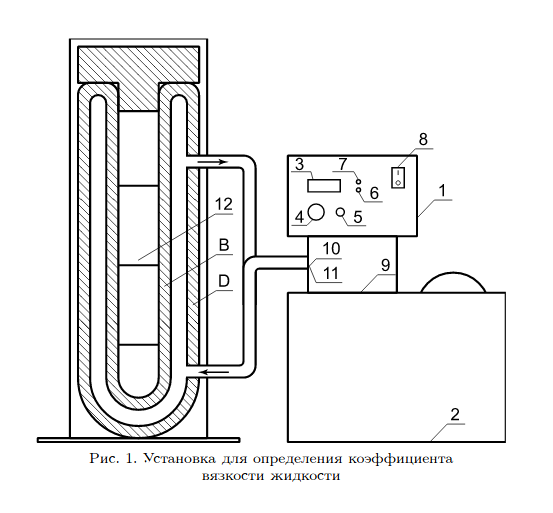
\includegraphics[width=0.95\textwidth]{equip.png}
\end{center}

\section*{Ход работы}
\subsection*{1}
Перед началом работы надо выбрать $\approx 10$ стальных и стеклянных шариков и промерить их диаметры (минимум два раза в различных направлениях, это делается для того, чтобы отбраковать несимметричные шарики (которых среди железных встречается примерно половиина)).
\subsection*{2}
4-5 раз надо повторить следующие шаги:
\begin{enumerate}
	\item выставить температуру на термостате
	\item подождать 5 минут для установления температурного равновесия
	\item выбрать 2 стальных и 2 стеклянных шарика, и каждый аккуратно окунуть в глицерин, замерив температуру прохождения щарика между 1-2 и 2-3 засечками.
\end{enumerate}
Шарики стоит опускать в воду с помощью пинцета, а также закрывать крышку сосуда с глицерином сразу после опускания шарика, для того, чтобы в глицерин не проникала влага из воздуха. Результаты эксперимента видны на таблице ниже:

\begin{center}
\begin{tabular}{|c|c|c|c|c|c|c|c|c|c|c|c|c|c|}\hline
Вещество&$T, ^\circ C$&$d, \text{мм}$&$t_0, \text{с}$&$t_1, \text{с}$&$\eta, 10\,\text{Па$\cdot$с}$&$\Delta \eta, 10\,\text{Па$\cdot$с}$
\\ \hline
сталь&$24.5$&$0.80$&$14.2$&$14.2$&$3.2$&$0.2$\\ \hline
стекло&$24.1$&$2.13$&$11.3$&$11.4$&$3.74$&$0.15$\\ \hline
стекло&$23.9$&$2.10$&$11.6$&$11.5$&$3.72$&$0.15$\\ \hline
сталь&$24.6$&$0.83$&$19.8$&$20.2$&$4.8$&$0.3$\\ \hline
сталь&$24.7$&$0.80$&$19.3$&$19.3$&$4.3$&$0.3$\\ \hline
стекло&$29.8$&$2.10$&$8.4$&$8.4$&$2.7$&$0.1$\\ \hline
стекло&$29.7$&$2.10$&$7.9$&$7.8$&$2.5$&$0.1$\\ \hline
сталь&$29.9$&$0.80$&$11.2$&$11.3$&$2.5$&$0.2$\\ \hline
сталь&$29.9$&$0.80$&$10.4$&$10.4$&$2.3$&$0.1$\\ \hline
стекло&$39.8$&$2.10$&$4.1$&$4.1$&$1.30$&$0.09$\\ \hline
стекло&$39.9$&$2.10$&$4.0$&$4.1$&$1.29$&$0.09$\\ \hline
сталь&$39.7$&$0.75$&$7.1$&$7.2$&$1.41$&$0.13$\\ \hline
сталь&$39.7$&$0.80$&$5.3$&$5.4$&$1.2$&$0.1$\\ \hline
стекло&$50.1$&$2.10$&$2.4$&$2.3$&$0.75$&$0.08$\\ \hline
стекло&$49.9$&$2.15$&$2.4$&$2.3$&$0.78$&$0.08$\\ \hline
сталь&$50.5$&$0.75$&$3.7$&$4.1$&$0.76$&$0.09$\\ \hline
сталь&$50.3$&$0.90$&$2.5$&$2.5$&$0.72$&$0.09$\\ \hline
стекло&$59.4$&$2.05$&$1.7$&$1.7$&$0.51$&$0.07$\\ \hline
стекло&$59.7$&$2.10$&$1.7$&$1.7$&$0.54$&$0.07$\\ \hline
сталь&$59.9$&$0.90$&$1.6$&$1.8$&$0.48$&$0.08$\\ \hline
сталь&$60.0$&$0.75$&$2.3$&$2.3$&$0.45$&$0.06$\\ \hline
\end{tabular}
\end{center}
$$\Delta T=0.2\, ^\circ C,\,\,\Delta d=0.025\, \text{мм},\,\,\Delta t_0=0.2\, \text{с},\,\,\Delta t_1=0.2\, \text{с}.$$

\subsection*{3}
Для каждого опыта надо вычислить число Рейнольдса $Re=\frac{\rho v r}{\eta}$, время релаксации $\tau = \frac{v}{g}$ и путь релаксации $s = \frac{v^2}{g}$ для того, чтобы понять, применимы ли наши предположения о том, что шарик мгновенно выходит на постоянную скорость ламинарного падения в жидкости. Как следует из таблицы ниже, число Рейнольдса не превосходит 0.2, что говорит о ламинарности течения жидкости в системе отчета шарика. Также видно, что шарик успевает выйти на постоянную скорость за миллисекунды, проходя при этом доли миллиметра, что говорит о том, что скорость шарика можно считать постоянной во время падения между засечками. Из этого можно сделать вывод, что формула
$$\eta=\frac{2}{9}gr^2\frac{\rho-\rho_\text{ж}}{v}$$
применима в нашей установке.
\newpage
\begin{center}
\begin{tabular}{|c|c|c|c|c|c|c|c|c|c|c|c|c|c|c|c|}\hline
Вещество&$T, ^\circ C$&$d, \text{мм}$&$t_0, \text{с}$&$t_1, \text{с}$&$10\,Re$&$\Delta 10\,Re$
&$\tau, \text{мс}$&$\Delta \tau, \text{мс}$
&$s, \text{мкм}$&$\Delta s, \text{мкм}$
\\ \hline
стекло&$24.1$&$2.13$&$11.3$&$11.4$&$0.065$&$0.004$&$0.899$&$0.015$&$7.9$&$0.2$\\ \hline
стекло&$23.9$&$2.10$&$11.6$&$11.5$&$0.063$&$0.004$&$0.882$&$0.015$&$7.6$&$0.2$\\ \hline
стекло&$29.8$&$2.10$&$8.4$&$8.4$&$0.12$&$0.01$&$1.22$&$0.02$&$14.6$&$0.6$\\ \hline
стекло&$29.7$&$2.10$&$7.9$&$7.8$&$0.14$&$0.01$&$1.30$&$0.03$&$16.7$&$0.8$\\ \hline
стекло&$39.8$&$2.10$&$4.1$&$4.1$&$0.51$&$0.06$&$2.5$&$0.1$&$61$&$6$\\ \hline
стекло&$39.9$&$2.10$&$4.0$&$4.1$&$0.52$&$0.07$&$2.5$&$0.1$&$62$&$6$\\ \hline
стекло&$50.1$&$2.10$&$2.4$&$2.3$&$1.6$&$0.3$&$4.4$&$0.3$&$186$&$31$\\ \hline
стекло&$49.9$&$2.15$&$2.4$&$2.3$&$1.5$&$0.3$&$4.4$&$0.3$&$186$&$31$\\ \hline
стекло&$59.4$&$2.05$&$1.7$&$1.7$&$3.1$&$0.8$&$6.1$&$0.7$&$362$&$86$\\ \hline
стекло&$59.7$&$2.10$&$1.7$&$1.7$&$3.0$&$0.8$&$6.0$&$0.7$&$355$&$83$\\ \hline
сталь&$24.6$&$0.83$&$19.8$&$20.2$&$0.033$&$0.003$&$0.510$&$0.005$&$2.55$&$0.05$\\ \hline
сталь&$24.7$&$0.80$&$19.3$&$19.3$&$0.037$&$0.004$&$0.529$&$0.005$&$2.74$&$0.05$\\ \hline
сталь&$29.9$&$0.80$&$11.2$&$11.3$&$0.109$&$0.014$&$0.91$&$0.01$&$8.1$&$0.2$\\ \hline
сталь&$29.9$&$0.80$&$10.4$&$10.4$&$0.13$&$0.01$&$0.98$&$0.01$&$9.5$&$0.3$\\ \hline
сталь&$39.7$&$0.75$&$7.1$&$7.2$&$0.29$&$0.04$&$1.43$&$0.03$&$20$&$1$\\ \hline
сталь&$39.7$&$0.80$&$5.3$&$5.4$&$0.48$&$0.08$&$1.90$&$0.07$&$35$&$2$\\ \hline
сталь&$50.5$&$0.75$&$3.7$&$4.1$&$1.0$&$0.1$&$2.63$&$0.13$&$68$&$6$\\ \hline
сталь&$50.3$&$0.90$&$2.5$&$2.5$&$1.9$&$0.4$&$4.0$&$0.3$&$158$&$24$\\ \hline
сталь&$59.9$&$0.90$&$1.6$&$1.8$&$4.3$&$1.3$&$6.1$&$0.7$&$359$&$85$\\ \hline
сталь&$60.0$&$0.75$&$2.3$&$2.3$&$2.8$&$0.7$&$4.5$&$0.3$&$195$&$34$\\ \hline
сталь&$24.5$&$0.80$&$14.2$&$14.2$&$0.068$&$0.008$&$0.72$&$0.01$&$5.05$&$0.14$\\ \hline
\end{tabular}
\end{center}
$$\Delta T=0.2\, ^\circ C,\,\,\Delta d=0.025\, \text{мм},\,\,\Delta t_0=0.2\, \text{с},\,\,\Delta t_1=0.2\, \text{с}.$$

\subsection*{4, 5}
Поскольку $\eta \sim e^{W/kT}$, построив график зависимости $ln(\eta)$ от $T^{-1}$, можно узнать энергию активации $W$ по угловому наклону:

Из графика видно, что зависимости $ln(\eta)$ от $1/T$ для стали и стекла линейные, и с коэффициентами наклона:
$$T_\text{а-сталь} = \frac{W}{k} = (6.2 \pm 0.4) \cdot 10^3 \text{К}.$$
$$T_\text{а-стекло} = \frac{W}{k} = (5.6 \pm 0.2) \cdot 10^3 \text{К}.$$
Этот результат был найден по МНК и имеет неполную погрешность. Для учета приборной погрешности, нужно добавить компоненты:
$$\delta T_\text{а} = \sqrt{\delta T_\text{а-стат}^2 + \left(\frac{<\Delta ln(\eta)>}{ln(\eta)_{max} - ln(\eta)_{min}}\right)^2 + \left(\frac{<\Delta 1/T>}{(1/T)_{max} - (1/T)_{min}}\right)^2}.$$
Из этого:
$$T_\text{а-сталь} = \frac{W}{k} = (6.2 \pm 0.5) \cdot 10^3 \text{К}.$$
$$T_\text{а-стекло} = \frac{W}{k} = (5.6 \pm 0.4) \cdot 10^3 \text{К}.$$

\begin{center}
\begin{tabular}{|c|c|c|c|c|c|c|c|c|c|c|}\hline
Вещество&$T, ^\circ C$&$\eta, \text{Па} \cdot \text{с}$&$\Delta \eta, \text{Па} \cdot \text{с}$
&$\frac{1000}{T}, \text{К}^{-1}$&$\Delta \frac{1000}{T}, \text{К}^{-1}$
&$ln(\frac{\eta} {1 \text{Па} \cdot \text{с}})$&$\Delta ln(\frac{\eta} {1 \text{Па} \cdot \text{с}})$
\\ \hline
стекло&$24.1$&$3.74$&$0.15$&$3.36$&$0.02$&$1.32$&$0.04$\\ \hline
стекло&$23.9$&$3.72$&$0.14$&$3.36$&$0.02$&$1.31$&$0.03$\\ \hline
стекло&$29.8$&$2.7$&$0.1$&$3.30$&$0.02$&$0.99$&$0.04$\\ \hline
стекло&$29.7$&$2.5$&$0.1$&$3.30$&$0.02$&$0.92$&$0.04$\\ \hline
стекло&$39.8$&$1.30$&$0.09$&$3.19$&$0.01$&$0.27$&$0.07$\\ \hline
стекло&$39.9$&$1.29$&$0.08$&$3.19$&$0.01$&$0.26$&$0.06$\\ \hline
стекло&$50.1$&$0.75$&$0.08$&$3.09$&$0.01$&$-0.2$&$0.1$\\ \hline
стекло&$49.9$&$0.78$&$0.07$&$3.09$&$0.01$&$-0.2$&$0.1$\\ \hline
стекло&$59.4$&$0.51$&$0.07$&$3.01$&$0.01$&$-0.67$&$0.14$\\ \hline
стекло&$59.7$&$0.5$&$0.2$&$3.00$&$0.01$&$-0.6$&$0.3$\\ \hline
сталь&$24.6$&$4.8$&$0.3$&$3.36$&$0.02$&$1.56$&$0.06$\\ \hline
сталь&$24.7$&$4.3$&$0.2$&$3.36$&$0.02$&$1.46$&$0.05$\\ \hline
сталь&$29.9$&$2.5$&$0.1$&$3.30$&$0.02$&$0.92$&$0.07$\\ \hline
сталь&$29.9$&$2.3$&$0.1$&$3.30$&$0.02$&$0.85$&$0.06$\\ \hline
сталь&$39.7$&$1.4$&$0.1$&$3.20$&$0.01$&$0.34$&$0.08$\\ \hline
сталь&$39.7$&$1.2$&$0.1$&$3.19$&$0.01$&$0.18$&$0.08$\\ \hline
сталь&$50.5$&$0.76$&$0.09$&$3.09$&$0.01$&$-0.2$&$0.1$\\ \hline
сталь&$50.3$&$0.72$&$0.08$&$3.09$&$0.01$&$-0.3$&$0.1$\\ \hline
сталь&$59.9$&$0.48$&$0.07$&$3.00$&$0.01$&$-0.73$&$0.15$\\ \hline
сталь&$60.0$&$0.45$&$0.15$&$3.00$&$0.01$&$-0.8$&$0.3$\\ \hline
сталь&$24.5$&$3.2$&$0.2$&$3.36$&$0.02$&$1.16$&$0.07$\\ \hline
\end{tabular}
\end{center}
$$\Delta T=0.2\, ^\circ C.$$

Из этого находим энергию активации, равную
$$W_\text{сталь} = k \cdot (6.2 \pm 0.5) \cdot 10^3\,\text{К} = 0.53\pm0.04\,\text{эВ},$$
$$W_\text{стекло} = k \cdot (5.6 \pm 0.4) \cdot 10^3\,\text{К} = 0.48\pm0.03\,\text{эВ},$$
что соответствует табличному значению
$$W_\text{табл} = 0.52\,\text{эВ}.$$
\begin{center}
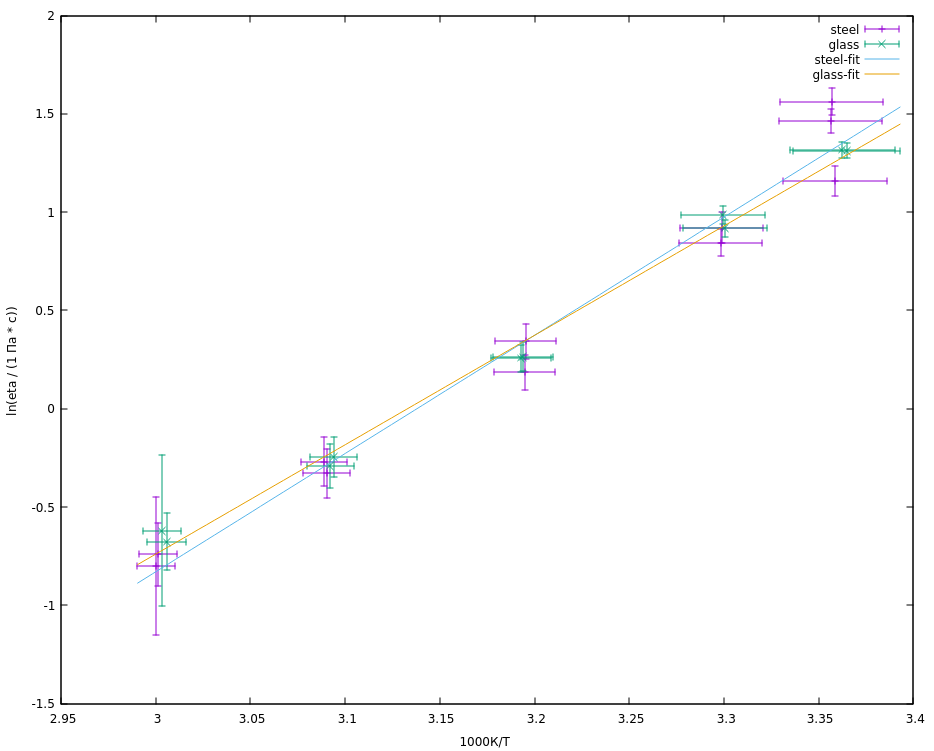
\includegraphics[width=0.95\textwidth]{plot.png}
\end{center}
\section*{Вывод}
Мы изучили новый метод измерения вязкости среды с помощью измерения скорости падающих в ней объектов, и с помощью него нашли температурную зависимость вязкости, из которой получили значение энергии активации глицерина. Полученная энергия активации сходится с табличным значением для каждого типа шариков.
\end{document}








\lipsum[1-4]
\begin{wrapfigure}{R}{5cm}
\centering
\includegraphics[width=0.20\textwidth]{rd.png}
\caption{1}
\end{wrapfigure}
\lipsum[1-6]


\begin{figure}[h]
\begin{center}$
\begin{array}{cccc}
\includegraphics[width=0.20\textwidth]{rd.png}&
\includegraphics[width=0.20\textwidth]{rd.png}&
\includegraphics[width=0.20\textwidth]{rd.png}&
\includegraphics[width=0.20\textwidth]{rd.png}\\
(1) & (2) & (3) & (4)
\end{array}$
\end{center}
\end{figure}
